% Numbered color palette. Reference swatches by their integer index when
% asking for a color in a figure. Mapping lives in `palette.txt`.
\documentclass[tikz,border=6pt]{standalone}
\usepackage{tikz}
\usepackage{xcolor}
\usetikzlibrary{calc}

\begin{document}
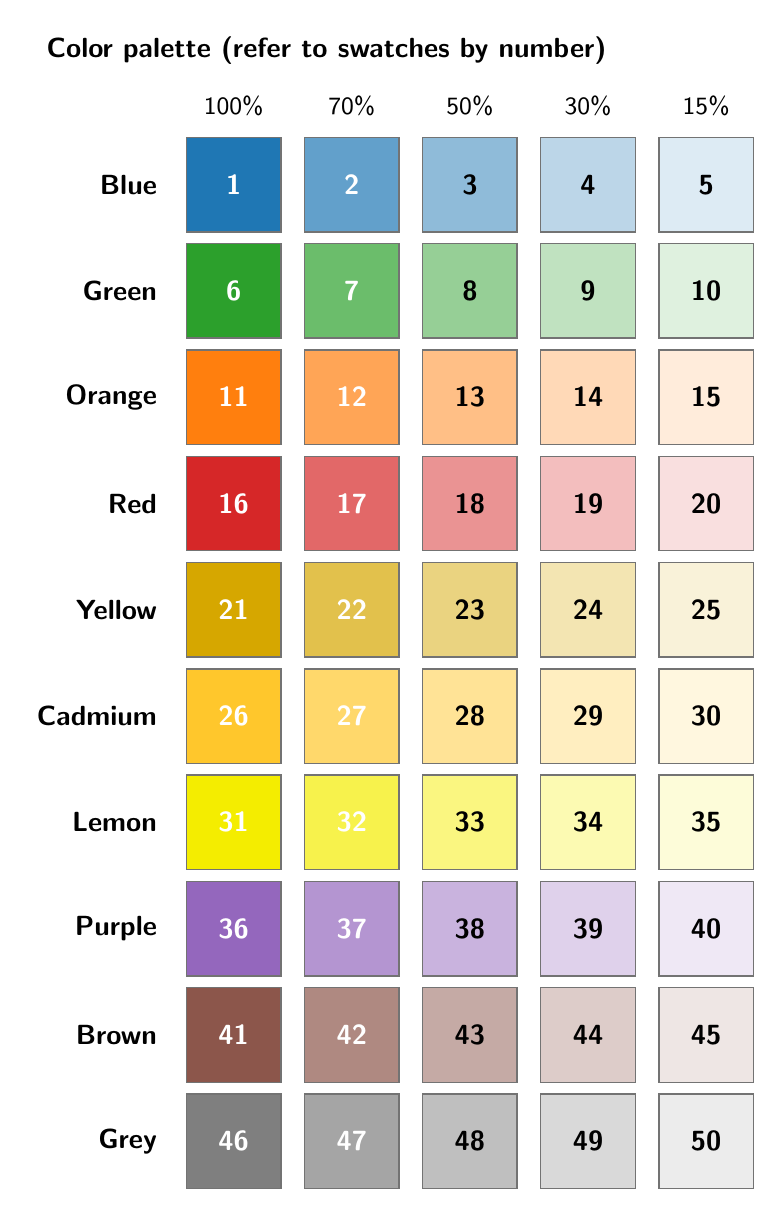
\begin{tikzpicture}[font=\sffamily\small]

% --- base colors (matplotlib tab10-ish) ---
\definecolor{cBlue}  {HTML}{1F77B4}
\definecolor{cGreen} {HTML}{2CA02C}
\definecolor{cOrange}{HTML}{FF7F0E}
\definecolor{cRed}   {HTML}{D62728}
\definecolor{cYellow}{HTML}{D6A700}    % goldenrod (original)
\definecolor{cCadm}  {HTML}{FFC72C}    % cadmium yellow (warm)
\definecolor{cLemon} {HTML}{F4ED00}    % lemon yellow (cool)
\definecolor{cPurple}{HTML}{9467BD}
\definecolor{cBrown} {HTML}{8C564B}
\definecolor{cGray}  {HTML}{7F7F7F}

% --- grid params ---
\pgfmathsetmacro{\sw}{1.20}
\pgfmathsetmacro{\gx}{1.50}
\pgfmathsetmacro{\gy}{1.35}

% --- lightness levels (5 columns) ---
\def\Lvls{100,70,50,30,15}

% --- column headers ---
\foreach \pct [count=\ci from 0] in \Lvls {
  \node[font=\sffamily\small, anchor=south]
       at (\ci*\gx, 0.75) {\pct\%};
}

% --- swatches + numbers ---
\foreach \fam/\famName [count=\ri from 0] in
  {cBlue/Blue, cGreen/Green, cOrange/Orange, cRed/Red,
   cYellow/Yellow, cCadm/Cadmium, cLemon/Lemon,
   cPurple/Purple, cBrown/Brown, cGray/Grey}{%
  \pgfmathsetmacro{\rowy}{-\ri*\gy}
  \node[anchor=east, font=\sffamily\bfseries]
       at (-0.85, \rowy) {\famName};
  \foreach \pct [count=\ci from 0] in \Lvls {%
    \pgfmathsetmacro{\idx}{int(\ri*5 + \ci + 1)}
    \pgfmathsetmacro{\cx}{\ci*\gx}
    \fill[\fam!\pct!white]
      (\cx-\sw/2, \rowy-\sw/2) rectangle (\cx+\sw/2, \rowy+\sw/2);
    \draw[black!55, line width=0.5pt]
      (\cx-\sw/2, \rowy-\sw/2) rectangle (\cx+\sw/2, \rowy+\sw/2);
    \pgfmathsetmacro{\useWhite}{ifthenelse(\pct>50, 1, 0)}
    \ifdim\useWhite pt=1pt
      \node[font=\sffamily\bfseries\normalsize, text=white] at (\cx,\rowy) {\idx};
    \else
      \node[font=\sffamily\bfseries\normalsize, text=black] at (\cx,\rowy) {\idx};
    \fi
  }
}

\node[anchor=south west, font=\sffamily\bfseries] at (-2.5, 1.4)
  {Color palette (refer to swatches by number)};

\end{tikzpicture}
\end{document}
